\chapter{Архитектура системы верификации}
В данной главе представлена архитектура системы верификации для синтеза и решения верификационных задач с использованием многоядерных и распределенных вычислительных систем.

\section{Компоненты системы верификации}
Подготовка и решение верификационных задач выполняются \textit{системой верификации}, для которой предлагается структура, представленная на рисунке~\ref{figure:system}. 
Система состоит из следующих компонентов:
\begin{itemize}
    \item сервер;
    \item решатель верификационных задач и заданий (далее решатель);
    \item генератор верификационных задач (далее генератор);
    \item инструменты верификации моделей программ.
\end{itemize}

\begin{figure}
\centering
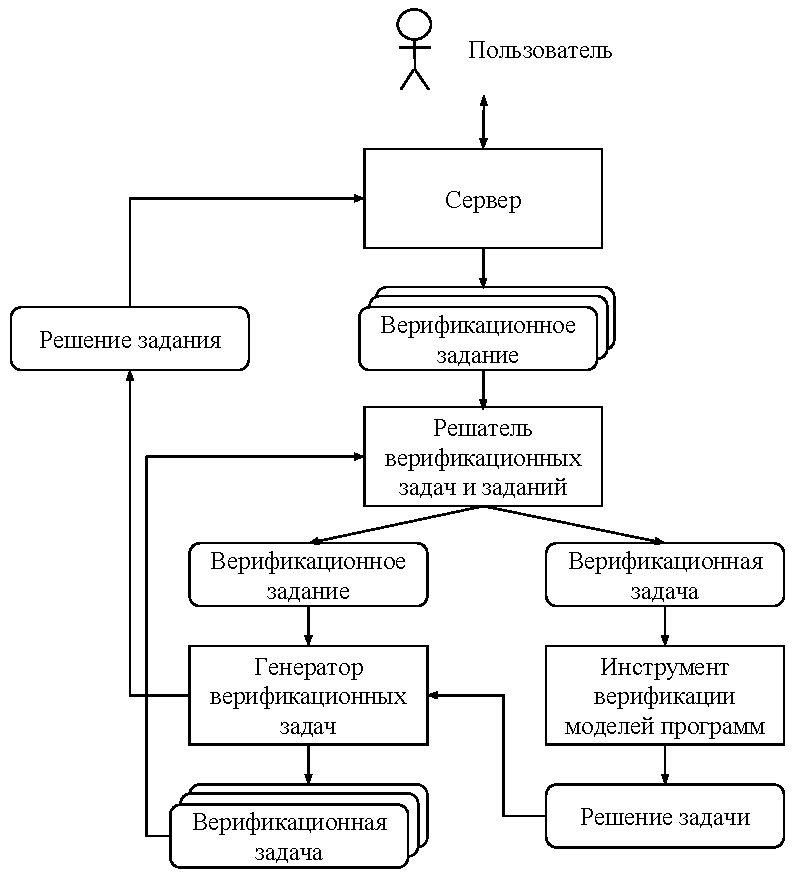
\includegraphics[scale=0.7]{system}
\caption{Структура системы верификации моделей программ.}
\label{figure:system}
\end{figure}

\section{Сервер}
Сервер выполняет следующие функции в рамках системы верификации:
\begin{itemize}
\item взаимодействие с пользователями;
\item организация взаимодействия между компонентами системы.
\item хранение результатов верификации; 
\end{itemize}

Пользователь взаимодействует с системой верификации через пользовательский интерфейс сервера.
Интерфейс предоставляет следующие функции:
\begin{itemize}
\item Позволяет создавать, изменять и удалять верификационные задания, которые содержат базу сборки программы, конфигурационные параметры и спецификации. 
Верификационное задание определяет ту часть программы, которая нуждается в проверке на соответствие заданным требованиям при определенных предположениях об окружении.
Верификационные задания могут включать десятки и сотни файлов, поэтому для каждой программы создается шаблон такого задания, а все последующие создаются пользователем при помощи его копирования и модификации.
\item Предоставляет возможность запуска и остановки решения верификационного задания, а также настройки ограничений на доступные при верификации вычислительные ресурсы. 
Пользователю должна быть доступна информация о всех решаемых верификационных заданиях, включая прогресс решения, оценку необходимого на завершение решения времени и полученные на текущий момент результаты.
Следует представлять пользователю информацию о статусе вычислительной системы, то есть объем доступных и используемых вычислительных ресурсов, подключенные узлы вычислительного кластера и их характеристики.
\item Реализует средства для экспертизы решений верификационных задач, включая оценку покрытия и предупреждений об ошибках.
\item Предоставляет инструменты для сравнения результатов решения верификационных заданий и переноса пользовательских оценок предупреждений об ошибках между результатами разными верификационных заданий, подготовленных для проверки требований к одной и той же программе.
\end{itemize}

В ходе работы между компонентами системы осуществляется активный обмен данными.
Верификационные задачи и задания между решателем и экземплярами генератора также передаются через сервер.
Данный компонент выполняет роль посредника между компонентами и надежного хранилища.
Такой подход позволяет избежать повторной передачи файлов, которые неоднократно могут отправляться компонентами.

В процессе верификации может накапливаться различная информация, которая может быть как получена автоматически в процессе верификации, так и подготовлена пользователем. 
Сервер предназначен для долговременного хранения полученных в ходе верификации артефактов в рамках верификационной системы.

\section{Генератор верификационных задач}
После того, как пользователь подготовил верификационное задание и инициировал его решение, оно попадает на вход решателю верификационных задач и заданий, который запускает экземпляр генератора верификационных задач.
Генератор выполняет подготовку верификационных задач согласно подходу, изложенному во второй главе. 
Кроме декомпозиции, синтеза моделей окружения и требований, композиции верификационной задач в формате, предложенном сообществом SV"~COMP, данный компонент выполняет дополнительные шаги: оценку прогресса решения верификационного задания, добавление атрибутов к верификационным задачам, отправку их решателю и ожидание результатов, первичную обработку решений верификационных задач и подготовку отчета о решении верификационного задания для его загрузки на сервер.

Атрибуты для верификационной задачи отражают ряд ее отличительных свойств, например, имя и версию программы, идентификатор проверяемого требования и т.п.
Атрибуты позволяют в пользовательском интерфейсе сравнивать результаты верификации, полученные в рамках различных верификационных заданий, и могут использоваться решателем при распределении вычислительных ресурсов.

Процесс подготовки верификационных задач может быть длительным, существенно превышающим время компиляции.
Поэтому подготовка задач должна выполняться параллельно и одновременно с их решением.
После декомпозиции программы на модули генератор верификационных задач выполняет шаги генерации верификационной задачи для каждого модуля независимо от остальных, поэтому этот процесс может быть естественным образом распареллелен.
Все генерируемые верификационные задачи отправляются затем решателю для запуска инструментов верификации моделей программ.

Результат решения каждой верификационной задачи состоит из вердикта, свидетельств нарушения или корректности, а также отчета о покрытии, который может быть подготовлен некоторыми инструментами верификации моделей программ.
Так как свидетельства нарушений об ошибках предназначены для валидации, а пользователю необходимо выполнять экспертизу сообщений об ошибках, то выполняется ряд преобразований свидетельств нарушений перед их отправкой на сервер:
\begin{itemize}
    \item Для каждой операции ошибочного пути в свидетельстве нарушения добавляется ссылка на модуль оригинального исходного кода программы, модели окружения или требования.
    Данное преобразование выполняется из-за того, что верификационная задача содержит препроцессированный, инструментированный срез исходного кода определенного модуля программы, который затруднительно анализировать пользователю.
    \item Помечаются операции ошибочного пути в зависимости от принадлежности оригинальному исходному коду программы или моделям окружения или требования.
    \item Добавляются аннотации на естественном языке для пользователя, чтобы объяснить модели событий сценариев взаимодействия в ошибочном пути, а также обосновать нарушение требования.
    \item Выделяются операции, либо релевантные проверяемому требованию, либо содержащие предположения инструмента верификации о неопределенных функциях, значениях переменных и памяти, которые могут оказаться неверными.
\end{itemize}

Покрытие выделяет ту часть программы, которая была проверена инструментом верификации моделей программ.
Хотя инструменты верификации проверяют все возможные пути выполнения в исходном коде верификационной задачи, неполная модель окружения, которая не содержит вызов определенных точек входа модуля, может привести к недостижимости некоторых фрагментов исходного кода.
Отчет о покрытии при верификации схож с отчетом о тестовом покрытии, но он может содержать и дополнительную информацию, например, предположения о диапазонах значений некоторых переменных, число состояний в модели программы для определенного участка верификационной задачи и т.д.
Следует выполнять аналогичные преобразования отчетов о покрытии, что были перечислены для свидетельств нарушений.
Отчеты о покрытии, полученные для разных верификационных задач для проверки одного и того же требования, могут быть объединены в единые итоговые отчеты.
Такой отчет передается генератором верификационных задач на сервер в составе отчета о завершении решения верификационного задания.

Решение верификационного задания может требовать много времени.
Например, система верификации LDV~Tools выполняет проверку драйверов одной версии ядра ОС Linux на соответствие одному требованию за время более суток, решая верификационные задачи последовательно.
Отправка результатов верификации во время решения верификационного задания параллельно с подготовкой и решением верификационных задач позволит на раннем этапе пользователю определить наличие ошибок в конфигурациях и спецификациях.

Обработку результатов решения верификационных задач также следует выполнять параллельно.
Решение каждой верификационной задачи не зависит от остальных, поэтому соответствующие отчеты о покрытии и свидетельства нарушений могут быть подготовлены независимо друг от друга и переданы на сервер.
Итоговые отчеты о покрытии и свидетельства нарушений после первичной обработки могут содержать файлы с исходным кодом программы, моделей требований и окружения.
Поэтому передача данных между сервером и экземплярами генератора верификационных задач должна минимизировать повторную передачу одних и тех же файлов, так как их число и размер могут быть достаточно велики.

\section{Решатель верификационных задач и заданий}
Верификационные задачи, подготовленные в процессе решения верификационного задания, поступают решателю для запуска необходимых инструментов верификации моделей программ.
Каждое верификационное задание и задача имеют максимальное ограничение на вычислительные ресурсы: объем доступных оперативной памяти и памяти на диске, время выполнения и процессорное время.
Ограничения необходимо соблюдать для получения воспроизводимых результатов верификации, поэтому, если инструмент верификации моделей программ или генератор верификационных задач превышают квоту выделенных им вычислительных ресурсов, они должны быть остановлены.
Для контроля за ограничениями потребления вычислительных ресурсов  предлагается использовать существующие решения, например, BenchExec~\cite{Beyer2016}.
Преимуществом применения BenchExec является наличие адаптеров для инструментов верификации моделей программ, делающих интеграцию и применение новых инструментов верификации менее трудоемкой.

Решатель верификационных задач и заданий предназначен для управления вычислительными ресурсами и планирования выполнения экземпляров других компонентов.
Задача управления вычислительными кластерами на сегодняшний день имеет множество решений и реализаций, пригодных для распараллеливания вычислительных задач разного вида, поэтому разрабатывать новый инструмент управления распределенной вычислительной системой избыточно.
В то же время облачные сервисы и системы управления вычислительными кластерами имеют разные функции и ограничения.
Например, в первой главе рассматривался облачный сервис Google App Engine, который позволяет распараллелить запуск инструментов верификации, но не позволяет задать необходимые для практического использования ограничения на вычислительные ресурсы.
Методы и инструменты выполнения облачных вычислений постоянно развиваются, поэтому система верификации не должна опираться в существенной степени на архитектуру какой-либо конкретной системы управления вычислительным кластером.
Поэтому предлагается реализовать отдельные модули в качестве адаптеров к той или иной системе распределенных вычислений в зависимости от ее функциональности:
\begin{itemize}
    \item модуль прогнозирования ограничения на максимальный объем оперативной памяти;
    \item модуль планирования для выбора вычислительного узла;    
    \item модуль запуска экземпляров инструментов верификации и генератора верификационных задач.
\end{itemize}

При решении верификационной задачи резервируется значительный объем оперативной памяти, чтобы соблюсти условие воспроизводимости результатов верификации.
На практике для верификации одного драйвера ОС Linux может требоваться резервирование порядка 10 ГБ оперативной памяти.
В то же время большая часть верификационных задач может требовать существенно меньшего объема вычислительных ресурсов, чем задано в максимальных ограничениях.
Модуль прогнозирования на основе статистики решения верификационных задач оценивает вероятное меньшее значение требуемой оперативной памяти для конкретной верификационной задачи.
Статистика решения верификационных задач собирается независимо для верификационных задач с определенными атрибутами.
При решении задачи подбора подходящего ограничения требуется минимизировать ошибку, иначе, если инструмент верификации потребует больше оперативной памяти, чем было задано в новом ограничении, верификационную задачу следует решать повторно уже с максимальным ограничением, что может занять десятки минут процессорного времени.

Модуль планирования либо выполняет распределение верификационных заданий и задач между узлами вычислительного кластера, либо передает их следующим модулям решателя в случае использования облачного сервиса с собственным планировщиком.
В случае самостоятельного планирования модуль решает следующую задачу: имеется некоторое количество узлов с определенными моделями процессоров, числом физических ядер, объемом оперативной и дисковой памяти; требуется разместить на вычислительных узлах для решения верификационные задачи и задания для минимизации общего времени решения верификационных заданий.
Всю оперативную память и физические ядра процессоров нельзя выделять для решения верификационных заданий, так как в этом случае может не остаться вычислительных ресурсов для решения верификационных задач, что приведет к бесконечному ожиданию запущенных экземпляров генератора.
Данная задача может быть решена при помощи простейшего жадного алгоритма, который будет гарантировать, чтобы для решения верификационных задач всегда оставалось доступно необходимое количество вычислительных ресурсов.
На практике могут быть реализованы различные алгоритмы, учитывающие разные аспекты планирования, например, приоритет решаемых верификационных заданий.

На последнем шаге модуль запуска либо отправляет верификационное задание или задачу в определенный облачный сервис, либо запускает необходимые экземпляры компонентов на заданном вычислительном узле с определенными ограничениями на вычислительные ресурсы.
Данный компонент должен поддерживать отмену решения верификационных заданий или задач, выполняя завершение всех дочерних процессов компонентов и сообщая модулю планирования об освобождении вычислительных ресурсов.
В случае ошибок журнал с их описанием должен быть отправлен на сервер для предупреждения пользователя.
